% kompilace xelatex prezentace.tex
% dokumentace k beameru: http://ftp.cvut.cz/tex-archive/macros/latex/contrib/beamer/doc/beameruserguide.pdf

% nastavení formátu prezentace 16:9
\documentclass[czech,aspectratio=169]{beamer}

\usepackage{polyglossia}
\setmainlanguage{czech}
\usepackage{ulem}
\usepackage{relsize}
\usepackage{xspace}
\newcommand{\Rplus}{\protect\hspace{-.1em}\protect\raisebox{.35ex}{\smaller{\smaller\textbf{+}}}}
\newcommand{\Cpp}{\mbox{C\Rplus\Rplus}\xspace}

% nastavení vzhledu
% další možnosti vzhledu viz https://hartwork.org/beamer-theme-matrix/
\usetheme{Boadilla}
\usecolortheme{dove}

% vzhled slajdů vnitřní téma (např. vzhled odrážek)
\useinnertheme{circles} %možnosti: default circles rectangles rounded inmargin
% vzhled slajdů vnější téma
\useoutertheme{default} %možnosti: default, miniframes, smoothbars, sidebar, split, shadow, tree, smoothtree, infolines

% zavedeme čvutí modou barvu
\definecolor{CVUT}{HTML}{0065BD}
% čvutí modou použijeme jako hlavní barvu prezentace
\setbeamercolor{structure}{bg=white,fg=CVUT}

% jako font prezentace nadefinujeme oficiální ČVUT písmo Technika
% https://www.cvut.cz/logo-a-graficky-manual  -- inforek, příhlášení přes celoškolské heslo
%\usepackage{fontspec}
%\setsansfont{Technika-Kniha}

% vypneme navigační panel beamer (pro zapnutí zakomentujeme)
\beamertemplatenavigationsymbolsempty{}

% vygenerujeme slajdy s poznámkami
%\setbeameroption{show notes}

% vygeneruje slajdy s poznámky vhodné pro promítání na dvou monitorech
%\usepackage{pgfpages}
%\setbeameroption{show notes on second screen}

% další balíčky
\usepackage[outputdir=build]{minted}
\usepackage{hyperref}
\usepackage{tikz}

% Údaje o prezentaci
\title[Nástroj pro konfiguraci a monitorování]{Nástroj pro konfiguraci a monitorování}
\subtitle{Bakalářská práce}
\institute[FIT ČVUT v Praze]{Fakulta informačních technologií \\ České vysoké učení technické v Praze}
\author[V. Kubernát]{Václav Kubernát \\ Vedoucí práce: Ing. Tomáš Čejka, Ph.D.}
\date{3. 5. 2019}
\titlegraphic{
\includegraphics[width=.1\textwidth]{logo-cvut}}


\begin{document}


\begin{frame}
    \titlepage{} %generuje se automaticky z section, subsection, subsubsection
    \note{Nezapomenout pozdravit}
\end{frame}

\begin{frame}
    \tableofcontents
\end{frame}

\section{Motivace}
\begin{frame}
\tableofcontents[currentsection]
\end{frame}
\begin{frame}{Existující konfigurační nástroje}
\begin{itemize}
\pause{}
\item\only<2>{grafické nástroje} \pause{}
\only<3->{\sout{grafické nástroje} -- nelze použít na mnoho zařízení najednou} \pause{}
\item Cisco IOS \pause{}
\item využití otevřených standardů
\end{itemize}
\end{frame}

\setbeamercovered{%
  again covered={\opaqueness<1->{15}}}
  \begin{frame}<1,2>[label=pozadavky]{Požadované vlastnosti aplikace}
      \begin{itemize}[<+>]
          \item konzole
          \item využívá otevřené standardy
          \item je intuitivní
      \end{itemize}
  \end{frame}

\begin{frame}{Konfigurační protokoly}
    \begin{itemize}
        \pause{}
        \item[] SNMP
            \begin{itemize}
                \item 1990
                \item nepodporuje transakce
            \end{itemize}
            \pause{}
        \item[] NETCONF
            \begin{itemize}
                \item 2011
                \item server-klient
                \item vytvořen společně s modelovacím jazykem YANG
                \pause{}
                \item klientskou část implementuje Netopeer2-cli
            \end{itemize}
    \end{itemize}
\end{frame}

\againframe<2,3>{pozadavky}


\begin{frame}[fragile]{Intuitivita}
    \begin{columns}
        \pause{}
        \begin{column}{.47\textwidth}
\verb|$ ed|

\pause{}
\verb||

\verb|?|

\pause{}
\verb|help|

\pause{}
\verb|?|

\pause{}
\verb|h|

\pause{}
\verb|Invalid address|

\pause{}
\verb|quit|

\verb|?|

\pause{}
\verb|exit|

\verb|?|
        \pause{}
        \end{column}
        \begin{column}{.47\textwidth}
\verb|~/example$|\pause{} \verb|ls|

\pause{}
\verb|file1  file2  file3|

\verb|~/example$|\pause{} \verb|echo Hello > file1|

\verb|~/example$|\pause{} \verb|cat fi| \pause{}

\verb|~/example$| \verb|cat file|
\pause{}
\verb|file1  file2  file3|

\verb|~/example$ cat file|\pause{}\verb|1|

\pause{}
\verb|Hello|
        \end{column}
    \end{columns}
\end{frame}

\section{Použitá řešení}
\begin{frame}
\tableofcontents[currentsection]
\end{frame}

\begin{frame}[plain]
\begin{center}
\color{CVUT}
\Large NETCONF
\end{center}
\end{frame}


\begin{frame}{NETCONF}
    Implementace celého protokolu může být náročná. Řešení: použití knihovny.
    \pause{}
    \vfill
    libnetconf2 -- knihovna implementující NETCONF
    \begin{itemize}
        \item napsaná v jazyce C
        \item CESNET
    \end{itemize}
\end{frame}

\begin{frame}[plain]
\begin{center}
\color{CVUT}
\Large Zpracovávání vstupu
\end{center}
\end{frame}

\begin{frame}{Zpracovávání vstupu}
    \begin{itemize}
        \item[] Použití prostředků jazyka \Cpp{}
            \pause{}
            \begin{itemize}
                \item jednoduché, nicméně nabízí to samé, co \textit{ed}
            \end{itemize}
        \pause{}
        \item[] Použití knihovny na editaci vstupní řádky
            \pause{}
            \begin{itemize}
                \item umožňuje doplňování příkazů
                \pause{}
                \item podporuje klávesové zkratky
                \pause{}
                \item použita knihovna \textit{replxx}
            \end{itemize}
    \end{itemize}
\end{frame}

\begin{frame}{Tok dat v aplikaci}
\begin{center}
    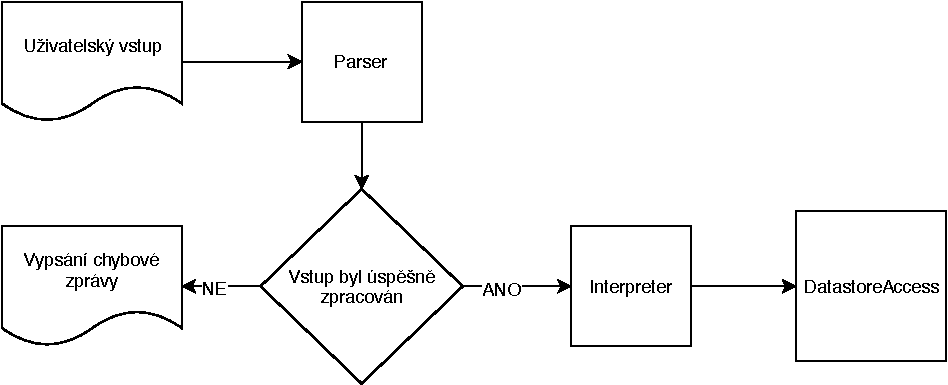
\includegraphics[width=.9\textwidth]{diagram}
\end{center}
\end{frame}

\section{Závěr}
\begin{frame}
\tableofcontents[currentsection]
\end{frame}

\begin{frame}<1,2,3>[fragile,label=porovnani]{Porovnání s \textit{Netopeer2-cli}}
    Změna hodnoty example:leafInt na 5.
    \vfill
    \begin{columns}
        \pause{}
        \begin{column}{.47\textwidth}
            \verb|// ... připojení k serveru ...|

            \verb|>|\pause{} \verb|edit-config --target --config|

            \pause{}
            \verb|OK|

            \verb|>|\pause{} \verb|commit|

            \pause{}
            \verb|OK|

            \verb|>|

        \end{column}
        \pause{}
        \begin{column}{.47\textwidth}
            \verb|// ... připojení k serveru ...|

            \verb|>|\pause{} \verb|set |

            \pause{}
            \verb|example:leafInt example:leafString|

            \verb|> set example:leaf|\pause{}\verb|I|\pause{}\verb|nt|\pause{} \verb|5|

            \pause{}
            \verb|>|\pause{} \verb|commit|

            \verb|>|
        \end{column}
    \end{columns}
\end{frame}

\begin{frame}[plain,fragile]
    \verb|    <!--#|

    \verb|    Type the content of the <edit-config>.|

    \verb|    -->|

    \color{gray}
    \verb|    ~|

    \verb|    ~|

    \verb|    ~|

    \verb|    ~|

    \verb|    ~|

    \verb|    ~|

    \verb|    ~|

    \verb|    ~|

    \verb|    ~|

    \verb|    ~|

    \verb|    ~|

\end{frame}

\againframe<4->{porovnani}

\begin{frame}{Shrnutí}
\begin{itemize}
\item[] Splnění požadavků:
    \begin{itemize}
        \pause{}
        \item konzolová aplikace\pause{} -- splněno
        \pause{}
        \item používá otevřený standard\pause{} -- splněno
        \pause{}
        \item nabízí prvky intuitivity\pause{} -- splněno
    \end{itemize}
    \pause{}
\item[] Možná rozšiřitelnost i na jiné protokoly, které používají YANG\@.
\end{itemize}
\pause{}
\vfill
Děkuji za pozornost.

\end{frame}
\end{document}
